\documentclass{fosuop} 

\usepackage{lipsum} %for dummy content, remove this

\makeglossaries % for list of abbreviations
\loadglsentries{prefatory-chapters/0-abbreviations} % Load abbreviations from file
\addbibresource{references.bib}

%variables
\def\projectTitle{\textless project title\textgreater}
\def\nameWithInitials{\textless john doe\textgreater}
\def\registrationNumber{\textless S/XX/XX\textgreater}
\def\departmentName{Department of Statistics and Computer Science}
\def\degreeName{BSc. (Honours) in Computer Science}
\def\universityName{University of Peradeniya}
\def\universityCountry{Sri Lanka}
\def\publicationYear{2023}
\def\supervisorNameOne{\textless supervisor one\textgreater}
\def\supervisorNameTwo{\textless supervisor two\textgreater}

\begin{document}

\title{}
\date{}
\author{}

\begin{titlepage}
    \begin{center}
    
    \begin{spacing}{1}
    {\fontsize{14pt}{0pt}\selectfont
    \textbf{\expandafter\MakeUppercase{\projectTitle}}}
    \end{spacing}
    
    \vspace{2.5cm}
    
    \textbf{\uppercase{a project report presented by}}
    
    \vspace{1.0cm}
    
    \begin{spacing}{1}
    \textbf{\uppercase{\expandafter\MakeUppercase{\nameWithInitials}}}
    \linebreak
    \textbf{\uppercase{\expandafter\MakeUppercase{(\registrationNumber)}}}
    \end{spacing}

    \vspace{1.0cm}
    
    \begin{spacing}{1.5}
    {to the Board of Study in}
    \linebreak
    \textbf{\expandafter\MakeUppercase{\departmentName}}
    
    \vspace{2.5cm}

    {\textit{ in partial fulfillment of the requirement \linebreak for the award of the degree of}}
    \end{spacing}
    
    \vspace{2.5cm}
    
    {\textbf{\degreeName}}
    
    \vspace{2.5cm}
    
    {of the}
    
    \vspace*{\fill}
    
    \begin{spacing}{1.5}
    {\expandafter\MakeUppercase{{\textbf{\universityName \linebreak \universityCountry \linebreak \publicationYear}}}}
    \end{spacing}
    
    \end{center}
    \thispagestyle{empty}
\end{titlepage}



\restoregeometry

\pagenumbering{roman}
\chapter*{Declaration}

\begin{spacing}{1}
I do hereby declare that the work reported in this project report/thesis was
exclusively carried out by me under the supervision of {\color{red} \supervisorNameOne}. It describes the results of my own independent research except where due reference has been made in the text. No part of this project report/thesis has been submitted earlier or concurrently for the same or any other degree. 

\vspace{2cm}

Date: ............................. \hspace*{\fill}..............................................
\newline
\hspace*{11cm} Signature of Candidate 

\vspace{2cm}

{\fontsize{11pt}{0pt}\selectfont
Certified by:

\vspace{1cm}

\begin{enumerate}
 \item Supervisor (Name):{\color{red} \supervisorNameOne} \hspace*{\fill} 
    Date: .................................
    
    \vspace{1.5cm}
    Signature:..............................................

    \vspace{2cm}

 \item Supervisor (Name):{\color{red} \supervisorNameTwo} \hspace*{\fill} 
    Date: .................................
    
    \vspace{1.5cm}
    Signature:..............................................
\end{enumerate}

}

\vspace{2cm}

{\fontsize{14pt}{0pt}\selectfont
\textbf{Department Stamp:} 
}

\end{spacing}

\newpage
\thispagestyle{plain}
\begin{spacing}{1}

\begin{center} 
    {\expandafter\MakeUppercase{\textbf{\projectTitle}}}

    \vspace{2em}

    {\textbf{\nameWithInitials}}

    \vspace{1em}

    {\fontsize{10pt}{0pt}\selectfont
        \departmentName, \universityName, \universityCountry
    }   
\end{center}

\vspace{2em}

{This paragraph should have the summary of the research with emphasis on the conclusions. This should fit in about three quaters of this page. This can have about 2-3 paragraphs} 
 
\end{spacing}

\chapter*{Acknowledgement}

Add acknowledgements and thanks in this chapter.



\renewcommand*\contentsname{Table of Contents}
\tableofcontents

\renewcommand{\listfigurename}{LIST OF FIGURES}
\listoffigures
\addcontentsline{toc}{chapter}{\listfigurename}

\renewcommand{\listtablename}{LIST OF TABLES}
\listoftables
\addcontentsline{toc}{chapter}{\listtablename}

% List of abbreviations
\printacronyms[title=list of abbreviations, toctitle=LIST OF ABBREVIATIONS, style=listofabbstyle]

\newpage
\pagenumbering{arabic}

\chapter{INTRODUCTION}\label{introduction}
\begin{spacing}{1.5}
  \lipsum[2-4]
\end{spacing}


\chapter{LITERATURE REVIEW}\label{lit-review}
\begin{spacing}{1.5}
\section{Citation demo}

This \textcite{dirac} citation is an example for text citation. The following shows a todo example. \todo{Write more details} Figure \ref{fig:colour_template_1} shows a colour template.

\begin{figure}[h]
	\centering
	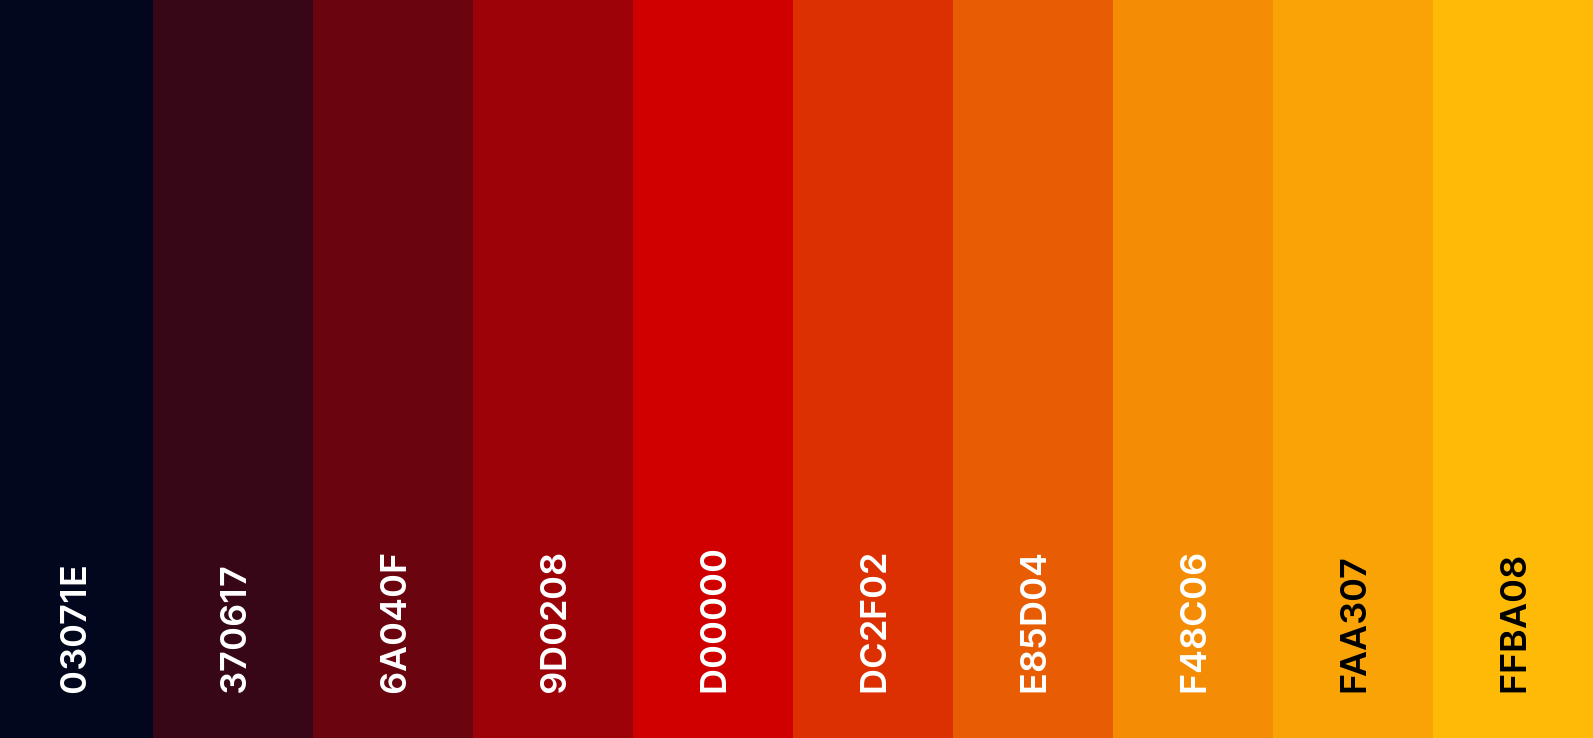
\includegraphics[width=0.7\textwidth]{images/example.png}
	\caption{Image 1}
	\label{fig:colour_template_1}
\end{figure}

\section{Abbreviation demo}

This is a demo for abbreviations \cite{dirac}. A section to test \cite{einstein} them.

\begin{figure}[h]
	\centering
	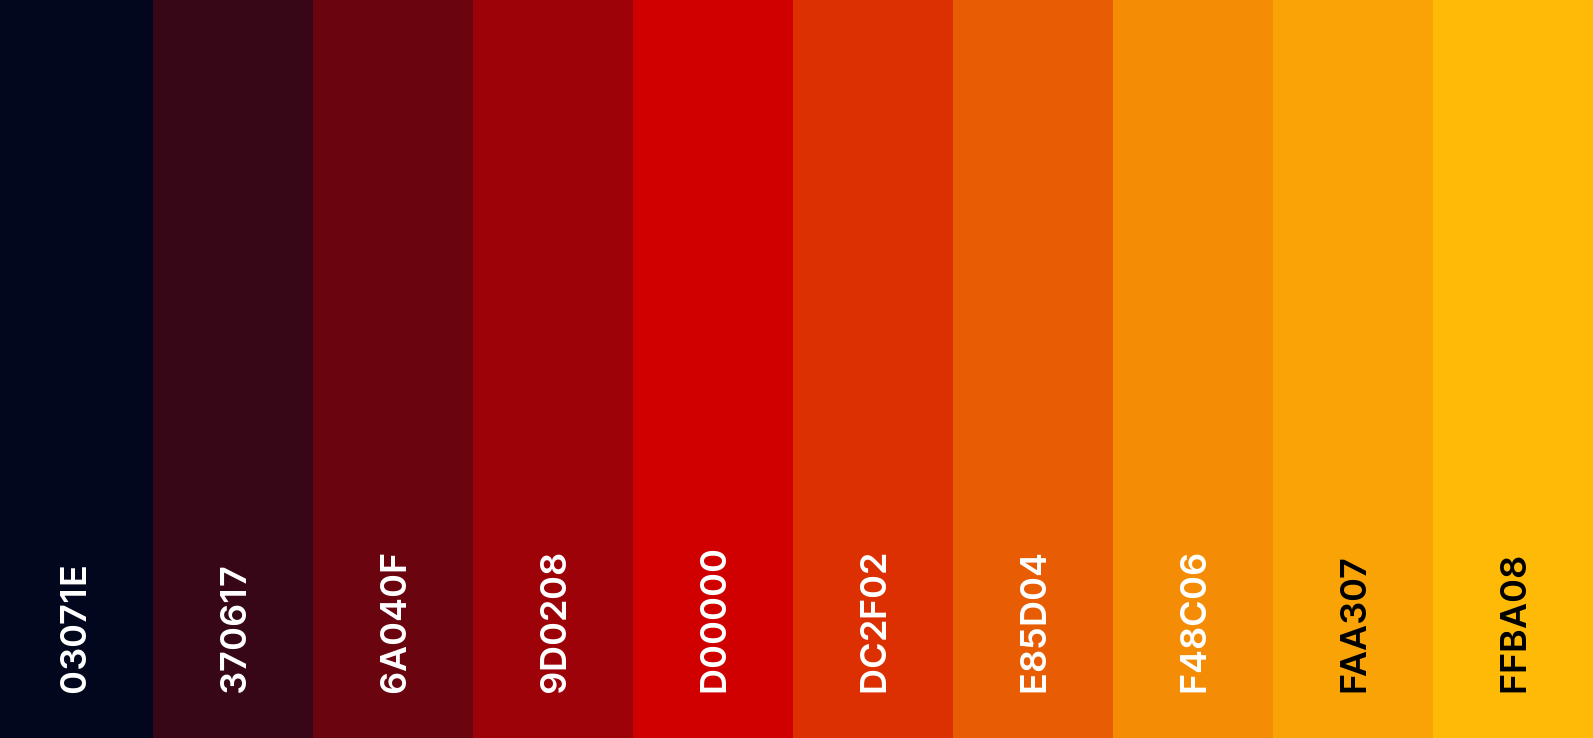
\includegraphics[width=0.7\textwidth]{images/example.png}
	\caption{Image 2}
	\label{fig:colour_template_2}
\end{figure}

This is an abbreviation demo for \gls{lcd}. Usage of the abbreviation the second time \gls{lcd}. The \gls{cpu} is the brain of the computer.
\end{spacing}


\chapter{DESIGN}\label{design}
\input{main-chapters/3-design}

\chapter{IMPLEMENTATION}\label{implementation}
\input{main-chapters/4-implementation}

\chapter{RESULTS AND DISCUSSION}\label{results}
\begin{spacing}{1.5}

\lipsum[2]
\begin{table}[h!]
    \centering
    \caption{\centering Trigonometric values}
    \label{tab:defence}
\begin{tabular}{|c|c|c|c|c|c|}
  \hline
  $\theta$ & $\sin(\theta)$ & $\cos(\theta)$ & $\tan(\theta)$ & $\cot(\theta)$ & $\sec(\theta)$ \\
  \hline
  $0^\circ$ & $0$ & $1$ & $0$ & N/A & $1$ \\
  \hline
  $30^\circ$ & $\frac{1}{2}$ & $\frac{\sqrt{3}}{2}$ & $\frac{1}{\sqrt{3}}$ & $\sqrt{3}$ & $\frac{2}{\sqrt{3}}$ \\
  \hline
  $45^\circ$ & $\frac{\sqrt{2}}{2}$ & $\frac{\sqrt{2}}{2}$ & $1$ & $1$ & $\sqrt{2}$ \\
  \hline
  $60^\circ$ & $\frac{\sqrt{3}}{2}$ & $\frac{1}{2}$ & $\sqrt{3}$ & $\frac{1}{\sqrt{3}}$ & $\frac{2}{\sqrt{3}}$ \\
  \hline
  $90^\circ$ & $1$ & $0$ & N/A & $0$ & N/A \\
  \hline
\end{tabular}
\end{table}

\end{spacing}


\chapter{CONCLUSION}\label{conclusion}
\begin{spacing}{1.5}
  \lipsum[2-4]
\end{spacing}


{\linespread{1}
	\printbibliography[title={REFERENCES},heading=bibintoc]}

\end{document}
